
\documentclass[letterpaper,oneside]{book}%

\usepackage[left=1in,right=2.75in,top=1in,bottom=1in]{geometry}
\marginparwidth 1.75in
\usepackage{etex}
\usepackage{tabls}
\usepackage{booktabs}
\usepackage{amsmath}
\usepackage{amssymb}
\usepackage{amsthm}
\usepackage{amsfonts}
\usepackage{pstricks}
\usepackage{multicol}
\usepackage{enumitem}
\usepackage{microtype}
\usepackage{makeidx}
%\usepackage{index}
\usepackage{tikz}
\usetikzlibrary{positioning,matrix,arrows,calc}
\tikzset{every picture/.style={>=latex,thick}}
\tikzset{grid lines/.style={semithick,dotted}}

\usepackage{pgfplots} 
\pgfplotsset{compat=1.3}
\usepgfplotslibrary{external}
\tikzexternalize
\tikzsetexternalprefix{figures/}

\newcommand{\remake}{\tikzset{external/force remake}}

\newcommand{\marginpartop}[1]{\marginpar{\vtop{%
  \vskip0pt
  \hbox{%
    #1%
  }%
}}}

\newcommand{\myscale}{1}

\usepackage{graphicx}
\usepackage{wrapfig}

\newcommand{\ds}{\displaystyle}
\newcommand{\dfdx}[1]{\frac{d#1}{dx}}
\newcommand{\ddx}{\frac{d}{dx}}

\usepackage{sagetex}


\let\oldmarginpar\marginpar
\renewcommand\marginpar[1]{\-\oldmarginpar{\raggedright\footnotesize #1}}
%\renewcommand\marginpar[1]{\-\oldmarginpar[\raggedleft\footnotesize #1]{\raggedright\footnotesize #1}}

\renewcommand{\thefootnote}{\roman{footnote}}
\newcommand{\note}[1]{\footnote{#1}\marginpar{\fbox{\textbf{\thefootnote}}}}
%%%%%%%To make all notes ignored, uncomment the following command.
\renewcommand{\note}[1]{}

%\usepackage[12hr]{datetime}
%\newdateformat{draftdate}{%
%\shortdayofweekname{\THEDAY}{\THEMONTH}{\THEYEAR}, %
%\THEDAY\ \shortmonthname[\THEMONTH] \THEYEAR}
%\draftdate
%\usepackage{eso-pic}
%\AddToShipoutPicture{\put(10,10){\small Draft: \today\ at \currenttime }}%--- version: \MakeUppercase{\svnInfoRevision}}}



\theoremstyle{plain}
\newtheorem{theorem}{Theorem}[chapter]
\newtheorem*{theorem*}{Theorem}
\newtheorem{lemma}[theorem]{Lemma}
\newtheorem*{lemma*}{Lemma}
\newtheorem{proposition}[theorem]{Proposition}
\newtheorem{corollary}[theorem]{Corollary}

\newtheoremstyle{box}%
{}{}% standard spacing before and after
{}% Body style
{}{\bfseries}{.}% Heading indent, font, and punctuation
{ }% space after heading
{\thmname{#1}\thmnumber{ #2}\thmnote{: #3}}% head spec


\theoremstyle{box}
\newtheorem{definition}{Definition}[chapter]
\newtheorem*{definition*}{Definition}
\newtheorem{observation}[theorem]{Observation}
\newtheorem{remark}{Remark}[chapter]
\newtheorem{example}{Example}[chapter]
\newtheorem{question}{Question}[chapter]
\newtheorem*{prep-problems}{Preparation Problems}

%\newcommand{\define}[2][]{\textit{#2}\index{#1#2}}
%\newcommand{\definemargin}[2][]{\marginpar{#2}\define[#1]{#2}}



% Abbreviations

\newcommand{\ii}{\ensuremath{\mathbf{\hat \imath}}}
\newcommand{\jj}{\ensuremath{\mathbf{\hat \jmath}}}
\newcommand{\kk}{\ensuremath{\mathbf{\hat k}}}
\newcommand{\vv}{\ensuremath{\mathbf{v}}}
\newcommand{\colvec}[1]{\ensuremath{\begin{bmatrix}#1\end{bmatrix}}}
\DeclareMathOperator{\rank}{rank}
\DeclareMathOperator{\rref}{rref}
\DeclareMathOperator{\vspan}{span}
\DeclareMathOperator{\trace}{tr}
\DeclareMathOperator{\proj}{proj}
\DeclareMathOperator{\curl}{curl}
\newcommand{\RR}{\ensuremath{\mathbb{R}}}


%%% Local Variables: 
%%% mode: latex
%%% TeX-master: t
%%% End: 

%The purpose of this code is to allow me to put lines in matrices so that I can create augmented matrices.
\makeatletter
\renewcommand*\env@matrix[1][*\c@MaxMatrixCols c]{%
  \hskip -\arraycolsep
  \let\@ifnextchar\new@ifnextchar
  \array{#1}}
\makeatother

\newcommand{\cl}[1]{  \begin{matrix}  #1  \end{matrix}  }
\newcommand{\bm}[1]{  \begin{bmatrix}  #1  \end{bmatrix}  }
\newcommand{\inv}{^{-1}}
\newcommand{\im}{\ensuremath{\text{im }}}
\newcommand{\R}{\mathbb{R}}
\providecommand{\norm}[1]{\lVert#1\rVert} 


%------------------------------------------------------------------------------------------------------------

\usepackage{hyperref}
%\makeindex

\begin{document}
\newgeometry{left=1in,right=1in,top=1in,bottom=1in}

\frontmatter
\title{Multivariable Calculus}
\author{Ben Woodruff\thanks{Mathematics Faculty at Brigham Young
    University--Idaho, \url{woodruffb@byui.edu}} \and Jason
  Grout\thanks{\mbox{Mathematics Faculty at Drake University, Des Moines,
    IA, \url{jason.grout@drake.edu}}}}
\date{Typeset on \today\\
\vfill

\includegraphics[height=1.3cm]{by-sa}
\vfill}
\maketitle
\thispagestyle{empty}

\noindent\copyright{ 2010 Ben Woodruff and Jason Grout.  Some Rights Reserved.\\

\bigskip

\noindent Except where otherwise noted, this work is licensed under the Creative Commons
Attribution-ShareAlike 3.0 United States License. To view a copy of
this license, visit 
\begin{center}
  \url{http://creativecommons.org/licenses/by-sa/3.0/us/}
\end{center}
or send a letter to Creative Commons, 171 Second Street, Suite 300,
San Francisco, California, 94105, USA.

\bigskip

\noindent Please attribute this work to:
\smallskip

Ben Woodruff, Mathematics Faculty at Brigham Young University--Idaho,
 \url{woodruffb@byui.edu}, and

\smallskip

 Jason Grout, Mathematics Faculty at Drake University, Des Moines, IA,
 \url{jason.grout@drake.edu}.

\vfill 

The source for this work is available at \url{http://github.com/jasongrout/multivariable-calculus}.
\vfill
}
\restoregeometry
\tableofcontents



%\chapter*{Preface}
%
%I would like to thank BYU-Idaho for the resources they have provided me to create this text.  

%\chapter{Introduction}
%
%The introduction is entered using the usual chapter command. Since
%the introduction chapter appears before the \verb|mainmatter| TeX
%field, it is again an unnumbered chapter. The primary difference
%between the preface and the introduction in this sample document
%is that the introduction will appear in the table of contents and
%the page headings for the introduction are automatically handled
%without the need for the \verb|markboth| TeX field. You may use
%either or both methods to create chapters at the beginning of your
%document. You may also delete these preliminary chapters.





\mainmatter


\chapter{Curves, Coordinates, and Differentials}

This chapter covers the following ideas. 


\begin{enumerate}

\item Model motion in the plane using parametric equations. In particular, how do you describe circles, ellipses, and lines using parametric equations.
\item Be able to convert between rectangular and polar coordinates. 
\item Graph polar functions in the plane. Find intersections of polar equations, and illustrate that not every intersection can be obtained algebraically (you may have to graph the curves).
\item Find derivatives, tangent lines, area, arc length, and surface area using parametric and polar equations.

\end{enumerate}


%%% Local Variables: 
%%% mode: latex
%%% TeX-master: "../multivariable-calculus"
%%% End: 




\section{Parametric Equations}

How can we describe motion in the plane?  One idea is to let $t$ represent time, and then write two equations $x=f(t),y=g(t)$ to describe the $(x,y)$ location of the point at any time $t$.  This gives us our first example of a mathematical ``function'' where we put in one value $t$ and get out two values $x$ and $y$.  This approach gives us a valuable way to study motion in the plane. The equations $x(t), y(t)$ are called parametric equations of a curve.

The parametric equations $x = \cos t, y=\sin t$ for $0\leq t\leq 2\pi$ describe motion along a circle of radius 1 in the plane.  You can convince yourself of this by plotting the points for various values of $t$ (make a $t,x,y$ table and start plotting points).  Alternatively, if you recall that $\cos^2 t+\sin^2 t = 1$, then you can replace $\cos t$ with $x$ and $\sin t$ with $y$ to obtain $x^2+y^2=1$, a Cartesian equation for a circle of radius 1.  Similarly you can show that $x=a\cos t, y=b\sin t$ for $0\leq t\leq 2\pi$ gives equations for an ellipse of the form $\frac{x^2}{a^2}+\frac{y^2}{b^2}=1$.  The graph of a function of the form $y=f(x)$ can always be written parametrically as $x=t,y=f(t)$, and then any equation we studied in first semester calculus can be analyzed using parametric equations. Using the identity $\cosh^2 x-\sinh^2 x =1$, the parametric equations $x=\cosh t,y=\sinh t$ give parametric equations for a hyperbola $x^2-y^2=1$, where $-\infty<t<\infty$. Because $\cosh x$ and $\sinh x$ trace out a hyperbola as parametric equations, they are called the hyperbolic trigonometric functions.  

To parametrize the line segment from $(1,2)$ to $(2,3)$, let's start by giving a Cartesian equation. The slope is $1/2$, so an equation is $y-2=\frac{1}{2}(x-1)$.  One option is to let $x=t$ and then $y=2+\frac{1}{2}(t-1)$. In this case, to get the curve to start at $x=1$ and end at $x=2$, we require $1\leq t\leq 2$. Another option is to let $t=\frac{1}{2}(x-1)$ or $x=1+2t$, and then $y-2=t$ or $y=2+t$. When $x=1$ we have $t=0$, and when $x=2$ we have $t=1/2$, so we require $0\leq t\leq 1/2$. There are infinitely many ways to parametrize the same curve.

We need to learn how to write parametric equations given a curve, and we need to learn how to find a Cartesian equation (remove $t$ from the equations) when we are given parametric equations.  In the textbook in 10.2, they give an example of the cycloid which leads to parametric equations. It is not crucial that you master the ideas behind a cycloid, rather that you learn how to parametrize curves. We will practice this idea in class all semester long. Obtaining a skill in parameterizing curves requires lots of practice. 

\subsection{Derivatives and Tangent lines}
How do you find the slope $\frac{dy}{dx}$ for a parametric curve?  The simple answer comes from the chain rule and essentially can be thought of as divide the top and bottom by $dt$, giving $\frac{dy}{dx} = \frac{dy/dt}{dx/dt}$. In other words, the derivative with respect to $x$ is found by dividing derivatives with respect to $t$.  This allows us to find tangent lines and more.  To find the second derivative $\frac{d^2y}{dx^2}$, we first find $dy/dx$ and then compute $d(dy/dx)/dt$ and divide it by $dx/dt$, namely 
$\ds \frac{d(\frac{dy}{dx})}{dx} = \frac{d(\frac{dy}{dx})/dt}{dx/dt}$ 
(again divide the top and bottom by $dt$). Often times people use dots to denote derivatives with respect to $t$, so we could write this as $dy/dx=\dot y/\dot x$.

As an example, consider the ellipse $x=\cos t, y=\sin t$. The derivatives with respect to $t$ are $\dot x = dx/dt = -\sin t$ and $\dot y= dy/dt=\cos t$. The derivative of $y$ with respect to $x$ is $dy/dx = \dot y/\dot x = \frac{\cos t}{-\sin t} = -\cot t$.  The derivative of $y'$ with respect to $t$ is $(-\cot t)' = \csc^2 t$. Dividing this by $\dot x = -\sin t$ gives $d^2y/dx^2 = \csc^3t$.  To find the tangent line to the curve at $t=\pi$, we compute  $x=\sqrt 2/2, y=\sqrt 2/2$, and $dy/dx = -\cot (\pi/4) = -1$. Using the point-slope form of a line, we have the tangent line as $(y-\sqrt 2/2) = -1 (x-\sqrt 2 /2)$.



\section{Polar Coordinates}

We now introduce a new coordinate system, the polar coordinate system.  This is just another way of referencing points in the plane.  We use {$r$ and {$\theta$ to reference points.  The distance from the origin to the point {$P$ is called {$r$, and the angle made by the positive {$ x $-axis and a ray from the origin through {$ P $ is called {$ \theta $.  The key equations $ x=r\cos\theta, y=r\sin\theta , x^2+y^2=r^2$ come directly from a right triangle with one vertex at the origin, another at the point $P$, and another directly above or below $P$ on the $x$-axis. 

The point $(r,\theta) =(2, \pi/2)$ represents the point $(x,y)=(0,2)$. The point $(r,\theta) =(3, \pi/4)$ represents the point $(x,y)=(3\frac{\sqrt{2}}{2},3\frac{\sqrt{2}}{2})$. Notice that the point $(1,\pi)$ in polar coordinates is the same as the point $(1,3\pi)$ or $(-1,-\pi)$ in polar coordinates.  The same $(x,y)$ point in the plane can be represented by infinitely many different polar coordinate pairs.
\subsection{Converting between polar and Cartesian coordinates and graphing}
The graph of $r=2$ is a circle of radius $2$ in the plane.  The graph of $\theta =  \pi/3$ is a straight line through the origin with angle of inclination $\pi/3$.  The line $x=4$ can be rewritten in polar coordinates as $r\cos\theta = 4$, or $r=4\sec\theta$.  The polar coordinate equation $r=2\sin\theta $ can be converted to rectangular coordinates by multiplying both sides by $r$, giving $r^2 = 2r\sin\theta$, and then using the key equations to obtain $x^2+y^2 = 2y$, which is the equation of a circle $x^2+y^2-2y+1=1$, or $x^2+(y-1)^2=1$ centered at $(0,1)$ of radius $1$ (I completed the square to complete this example). The key equations will allow you to convert from one system to another. You may need to multiply both sides of an equation by $r$ to do a conversion (as in the last example).

To plot a polar equation, we just make an $r,\theta, x,y$ table and start plotting points.  You will discover after some practice that there are symmetries that you can use to help you learn how to plot polar curves.  To plot the curves by hand, try putting in values of $\theta$ which are on the unit circle, in particular use $0,\pi/2,\pi,3\pi/2$.  When you connect dots on your graphs, realize that you wrap around counter-clockwise as theta increases, and the variable $r$ that is changing is the distance from the origin.  Some common curves are shown below:

\newcommand{\mywidth}{1.3in}
\begin{center}
\begin{tabular}{cccc}
%polar_plot(cos(3*x),(x,0,2*pi),color='black',aspect_ratio=1).save('rose.pdf',aspect_ratio=1)
%polar_plot(2*cos(x)+1,(x,0,2*pi),color='black',aspect_ratio=1).save('limacon.pdf',aspect_ratio=1)
%polar_plot(1-cos(x),(x,0,2*pi),color='black',aspect_ratio=1).save('cardioid.pdf',aspect_ratio=1)

% cosines = [cos(-pi/2+pi*i/100) for i in range(201)]
% v = [(1/c, tan(-pi/2+pi*i/100)) for i,c in enumerate(cosines) if c != 0]
% L = [(a/(a^2+b^2), b/(a^2+b^2)) for a,b in v]
% p = line(L, color='black')
% p.save('lemniscate.pdf',aspect_ratio=1)

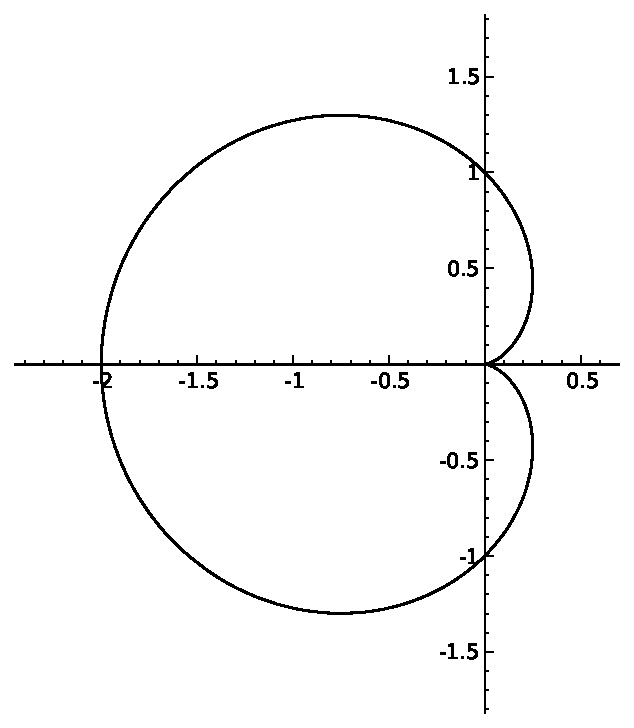
\includegraphics[width=\mywidth]{01-Curves-Coordinates-Differentials/cardioid}&
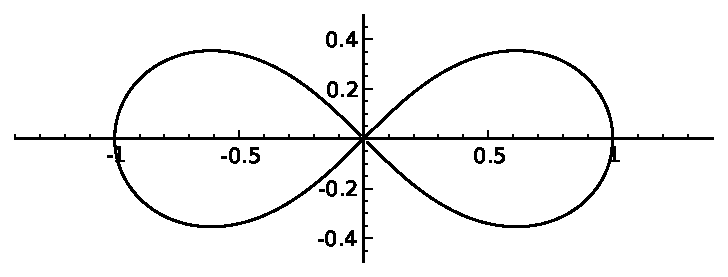
\includegraphics[width=\mywidth]{01-Curves-Coordinates-Differentials/lemniscate}&
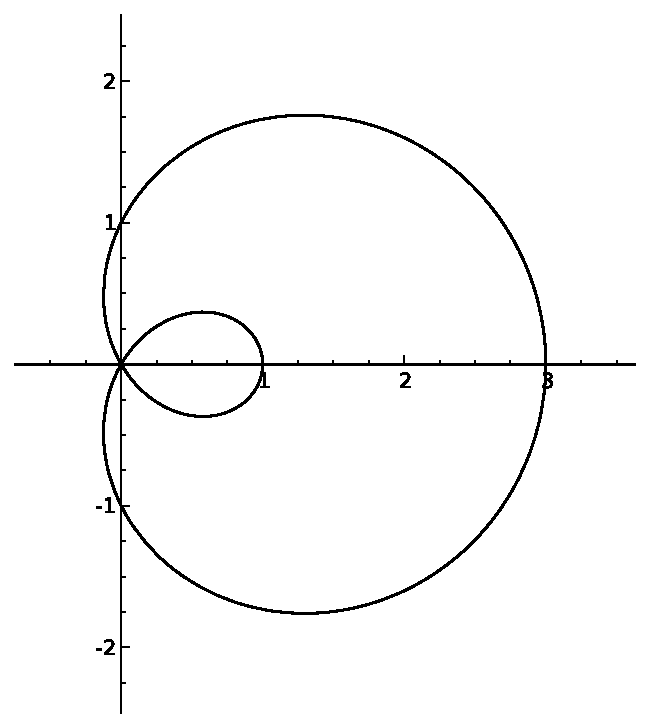
\includegraphics[width=\mywidth]{01-Curves-Coordinates-Differentials/limacon}&
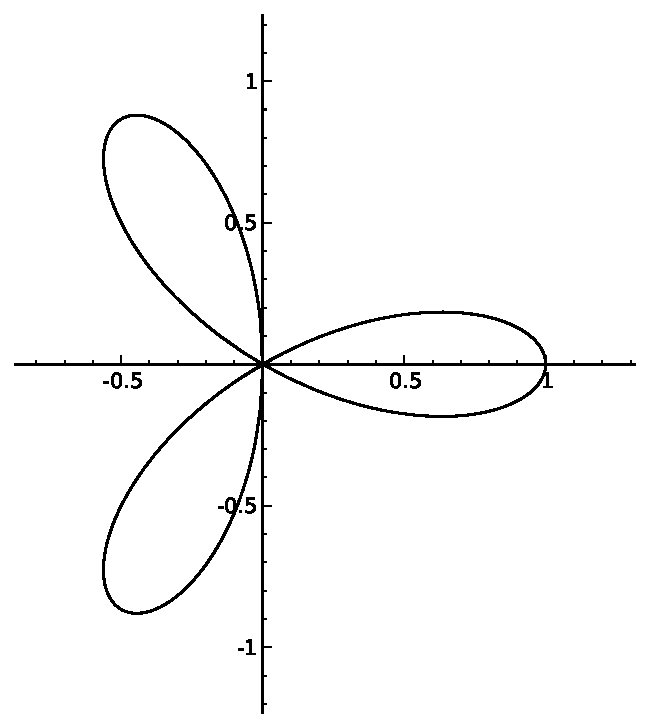
\includegraphics[width=\mywidth]{01-Curves-Coordinates-Differentials/rose}
\\
Cardioid&
Lemniscate&
Limacon&
Rose
\\
$r=1-\cos\theta$&
$r^2=\sin 2\theta$&
$r=2\cos\theta+1$&
$r=\cos 3\theta$
\end{tabular}
\end{center}

\subsection{Finding Intersections}
One problem with finding the intersection of two polar graphs is that there are many ways to represent the same point in polar coordinates.  Hence, when you solve for the intersection of two polar graphs, you may not find all the intersection points algebraically. Often you must graph the polar curves in addition to finding the points of intersection.  For example, the two curves $r=1-\cos\theta$ (a cardioid) and $r=\cos\theta$ (a circle of radius 1/2 centered at (1/2,0)) intersect in three points.  Solving for $\theta$ we have $\cos\theta = 1-\cos\theta$, or $2\cos\theta = 1$, or $\cos\theta = \frac{1}{2}$.  This occurs when $\theta = \pm \frac{\pi}{3}$. Hence the two points of intersection are $(x,y)=(r\cos\theta,r\sin\theta) = (1/4,\pm\sqrt 3 / 4)$.  The algebraic solution misses completely the fact that $(x,y)=(0,0)$ is an intersection point of the two graphs. It is best to graph any polar curves when you wish to find their intersection.



\section{Calculus and Differentials}

\subsection{Slope}
If a curve is given parametrically as $x=f(t),y=g(t)$, then we can find $\ds\frac{dy}{dx}$ using the chain rule. Symbolically we just divide both $dx$ and $dy$ by $dt$, and obtain $\ds\frac{dy}{dx} = \ds\frac{dy/dt}{dx/dt}$.  For example, if $x=3t$ and $y=t^2-t$, then $\ds\frac{dy}{dx} = \ds\frac{dy/dt}{dx/dt}=\frac{2t-1}{3t}$.  This is how we find the slope of graphs of parametric curves.

If the curve is given by a polar coordinate equation $r(\theta)=f(\theta)$, then we use the same principle.  Recall $x=r\cos\theta = f(\theta)\cos\theta$ and $y=r\sin\theta = f(\theta)\sin\theta$.  Hence we have 
$\ds\frac{dy}{dx} 
= \ds\frac{dy/d\theta}{dx/d\theta} 
= \frac{\frac{d}{d\theta} f(\theta)\sin\theta }{\frac{d}{d\theta} f(\theta)\cos\theta } 
= \frac{f^\prime (\theta)\sin\theta +f(\theta)\cos\theta }{ f^\prime(\theta)\cos\theta - f(\theta)\sin\theta} 
$. Don't worry about memorizing this formula, rather realize that it is just $\ds\frac{dy/d\theta}{dx/d\theta}$.





\subsection{Area Differential $dA$}

To find the area swept out by a segment from the origin to a polar curve, we first need to recall that the area of a sector of a circle is $\displaystyle \frac 12 r^2 \theta$. To derive this, just recall the area of a circle is  $\pi r^2$. So half a circle has area $\displaystyle \frac{\pi}{2}r^2$. If you sweep out $\theta$ radians, then you have covered $\displaystyle \frac{\theta}{2\pi}$ percent of the circle. So the area covered is $\displaystyle \frac{\theta}{2\pi}\cdot \pi r^2$.  

Now we take the simple formula, $\displaystyle \frac 12 r^2 \theta$ and use it to derive the integral formula $ \int_\alpha^\beta \frac 12 r^2 d\theta.$ Consider the region swept out by a segment from the origin to the polar curve $r=f(\theta)$ as $\theta$ ranges from $\alpha$ to $\beta$. Break up the region into small sectors, each having interior angle $\Delta \theta$. By making $\Delta \theta$ small enough, we can approximate the area $\Delta A_i$ of each sector by assuming the radius is constant, $f(\theta_i)$.  This gives $\Delta A_i\approx \frac12 f(\theta_i)^2 \Delta \theta$. To find the total area, we add up all the little areas and take a limit as $\Delta \theta\to 0$, as follows: $$A = \lim_{\Delta \theta\to 0} \sum\Delta A_i
=\lim_{\Delta \theta\to 0} \sum\frac12 f(\theta_i)\Delta \theta
=\int_\alpha^\beta \frac12 f(\theta)^2d \theta
=\int_\alpha^\beta \frac12 r^2d \theta.
$$
We use the differential notation 
$dA=\frac{1}{2}r^2d\theta$ to remember the integration formula.  If you can remember the area of a sector of a circle, then you can remember the integration formula.  You probably recall already the differential notation
$dA=f(x)dx$
To find area, all you have to do is remember that area is the integral of the area differential $dA$, so $A=\int dA = \int_a^b f(x)dx = \int_\alpha^\beta\frac{1}{2}r^2d\theta. $ To find area between two polar curves, just find the area inside the outer curve, and subtract the area inside the inner curve. The area inside the cardioid $r=1-\cos\theta$ is given by $\int_0^{2\pi}\frac{1}{2}(1-\cos\theta)^2d\theta$, which we would let a computer calculate for us.
 
\subsection{Arc Length Differential $ds$}


Finding length ({$\Delta s$}) along a straight line is done by finding the change in {$x$} (called {$\Delta x$}) and the change in {$y$} ({$\Delta y$}), and then using the Pythagorean identity to get {$\Delta s = \sqrt{\Delta x^2+\Delta y^2}$}. If a curve is not straight, then start by breaking the curve up into a bunch of small pieces of length {$\Delta s_i$}.  Along each small piece, the curve is approximately straight, so we approximate each {$\Delta s_i$} with {$\sqrt{\Delta x_i^2+\Delta y_i^2}$}. In differential notation this becomes $ds = \sqrt{dx^2+dy^2}$.  To find arc length {$s$}, we add up ({$\sum ds$}) the little pieces of arc length and take a limit to get {$s = \int_C ds = \int_C\sqrt{dx^2+dy^2}$}.  For a function $y=f(x), a\leq x\leq b$ whose independent variable is $x$, you can multiply $ds$ by $1=\frac{dx}{dx}$ to obtain $ ds = \sqrt{dx^2+dy^2}\frac{dx}{dx} = \sqrt{\left(\frac{dx}{dx}\right)^2+\left(\frac{dy}{dx}\right)^2}dt=\sqrt{1+\left(\frac{dy}{dx}\right)^2}dt$ which means arc length is $ s=\int_C ds = \int_a^b \sqrt{1+\left(\frac{dy}{dx}\right)^2}dx$. Similarly, for $x=g(y), c\leq y\leq d$ we multiply by $\frac{dy}{dy}$ to obtain
$ \int_c^d \sqrt{\left(\frac{dx}{dy}\right)^2+1}dy$. For 
parametric equations $x(t),y(t), a\leq t\leq b$ we multiply by $\frac{dt}{dt}$ to obtain $ \int_a^b \sqrt{\left(\frac{dx}{dt}\right)^2+\left(\frac{dy}{dt}\right)^2}dt$. 
The polar coordinate version $\int_\alpha^\beta \sqrt{r^2+\left(\frac{dr}{d\theta}\right)^2}d\theta$ comes from the nontrivial simplification $\left(\frac{dx}{d\theta}\right)^2+\left(\frac{dy}{d\theta}\right)^2 = r^2+\left(\frac{dr}{d\theta}\right)^2$, where $x=r\cos \theta, y=r \sin\theta$. 
Hence, to find the arc length for parametric or polar curves, we just integrate the arc length differential.


\subsection{Surface Area Differential $d\sigma$ (of a surface of revolution)}
When you revolve a curve about a line, the radius of rotation is the distance to the line. We will now develop formulas for find the surface area of a surface of revolution given by rotating about a line. 

Start by breaking the curve up into small pieces (as done before). The length of each piece is approximately given by the arc length approximate {$\Delta s_i$, which is a straight line segment from one end of the small portion of the curve to the other. We assume that the radius is constant, namely the distance {$radius_i$ to the line. 
If we rotate about the $x$-axis, then $radius_i=y_i$.  
If we rotate about the $y$-axis, then $radius_i=x_i$.
The surface area of a frustrum of a cone is $\Delta \sigma_i = 2\pi radius_i \Delta s_i$ (we use $\sigma$ to designate surface area). Adding each small pieces of surface area up $\sigma=\displaystyle \sum \Delta\sigma_i$, we get the integration formulas $\displaystyle
\sigma = \int d\sigma
= \int 2\pi\ radius\ ds
= \int_a^b 2\pi\ radius\ \sqrt{\left(\frac{dx}{dt}\right)^2+\left(\frac{dy}{dt}\right)^2}dt
= \int_\alpha^\beta 2\pi\ radius\ \sqrt{r^2+\left(\frac{dr}{d\theta}\right)^2}d\theta
.$
Note that if you can remember $d\sigma = 2\pi\ radius\ ds,$
then you just have to know what the radius is, and what to use for $ds$.  


The surface area of a surface of revolution formed by revolving a polar curve about the $x$-axis is given by the formula  $\ds \int_\alpha^\beta 2\pi |y| ds =
\int_\alpha^\beta 2\pi r\sin\theta \sqrt{r^2+\left(\frac{dr}{d\theta}\right)^2}d\theta$, provided $y\geq 0$.
When we revolve about the $y$-axis we obtain instead the formula 
$\ds \int_\alpha^\beta 2\pi |x| ds=
\int_\alpha^\beta 2\pi r\cos\theta \sqrt{r^2+\left(\frac{dr}{d\theta}\right)^2}d\theta$, provided $x\geq 0$.

If we rotate about a line such as $x=3$, then the distance to the line $x=3$ is given by $|x-3|$, so our formula is  $\ds \int_\alpha^\beta 2\pi |x-3| ds =
\int_\alpha^\beta 2\pi (r\cos\theta -3) \sqrt{r^2+\left(\frac{dr}{d\theta}\right)^2}d\theta$, provided $x\geq 3$ (otherwise we just leave the absolute values in the problem).

%%% Local Variables: 
%%% mode: latex
%%% TeX-master: "../multivariable-calculus"
%%% End: 






\newgeometry{left=1in,right=1in,top=1in,bottom=1in}
\newpage

\section{Preparation}

\noindent
This chapter covers the following ideas. When you create your lesson plan, it should contain examples which illustrate these key ideas. Before you take the quiz on this unit, meet with another student out of class and teach each other from the examples on your lesson plan. 


\begin{enumerate}

\item Model motion in the plane using parametric equations. In particular, how do you describe circles, ellipses, and lines using parametric equations.
\item Be able to convert between rectangular and polar coordinates. 
\item Graph polar functions in the plane. Find intersections of polar equations, and illustrate that not every intersection can be obtained algebraically (you may have to graph the curves).
\item Find derivatives, tangent lines, area, arc length, and surface area using parametric and polar equations.

\end{enumerate}


%%% Local Variables: 
%%% mode: latex
%%% TeX-master: "../multivariable-calculus"
%%% End: 



\subsection{Preparation and Homework Suggestions}

Most class sessions will begin with us presenting prepared material
(``Preparation problems'') in groups.  Typically there will be 4
preparation problems assigned for each day. Each member of the group
should prepare one of these problems before class and teach the rest
of the group what is needed to complete this problem. You will
occasionally select a problem which is entirely new to you, which you
have never seen modeled before. When this occurs, you should look for
examples similar to this problem in the text to learn how to do the
problem. You will grow in skill and in confidence as you study and
prepare these new preparation problems. The new problem will normally
be the last one listed in the preparation problems, so I suggest that
as a group you alternate who takes this problem so that everyone has a
chance to grow this way.


\begin{center}
\begin{tabular}{ll}
&Preparation Problems\\
\hline\hline
Day 1& 10.2:8, 10.2:51, 10.2:66, 10.2:69
\\\hline
Day 2& 10.3:7, 10.3:76, 10.3:99
\\\hline
\end{tabular}
\end{center}

 In the
following list, the ``basic practice'' problems should be quick
problems to help you master the ideas.  The ``good problems'' will
require a little more work.  The theory and application problems are
ones that will challenge you more; make sure you do the problems from
this area to fully master the material.
\medskip
{\noindent \footnotesize 
\begin{tabular}{|l|c|l|l|l|l|}\hline
Topic &Sec &Basic Practice &Good Problems &Thy/App \\\hline
Parametric Equations & 10.2 & 1--32 & 33--37, 39--40, 43--46, 51--62 & 38, 63-66, 67--72 \\\hline
Calculus of Parametric Equations & 10.3 & 1--16, 43--52, 63--66 & 17--42, 53--56, 67--72 & 57--100 \\\hline
Polar coordinates & 10.4 & 1-21, 23--42, 73--80 & 43--53, 59--60 & 54--58, 81--92\\\hline
Area and arclength & 10.5 & 1--26, 45--48 & 27--30, 31--40& 41--44, 69--77\\\hline

\end{tabular}
\smallskip
}

Don't worry about trying to solve by hand all of the integrals for calculating arc length, surface area, etc..  If you can set them up, and solve the simpler ones, you are doing great.


%%% Local Variables: 
%%% mode: latex
%%% TeX-master: "../multivariable-calculus"
%%% End: 


%%% Local Variables: 
%%% mode: latex
%%% TeX-master: "../multivariable-calculus"
%%% End: 

\restoregeometry



\chapter{Vectors}

This chapter covers the following ideas. 

% A list of objectives for the chapter
%\begin{enumerate}
%\item ...
%\end{enumerate}

\begin{enumerate}
\item Define, draw, and explain what a vector is in two and three
  dimensions.
\item Add, subtract, multiply (scalar, dot, and cross product)
  vectors. Be able to illustrate each operation geometrically.
\item Use vector products to find angles, length, area, projections,
  and work.
\item Use vectors to give equations of lines and planes and be able to
  draw lines and planes in 3D.
\end{enumerate}



%%% Local Variables: 
%%% mode: latex
%%% TeX-master: "../multivariable-calculus"
%%% End: 


\section{Multiple dimensions}
Before plotting points in three dimensions, we need to establish
conventions about the axes. The most common method of graphing is to
use a right-hand coordinate system.  Your right pointer finger
represents the positive {$x$}-axis, your middle finger represents the
positive {$y$}-axis, and your thumb represents the positive
{$z$}-axis.  Your hand represents the origin (the point $(0,0,0)$).
To plot a point in 3D, it's helpful to visualize a rectangular box
with one corner at the origin and the opposing corner at the point of
interest.

%\begin{example}
%  \note{plot the boxes representing (1,2,3) and (-1,4,-2)}
%\end{example}

We use the Pythagorean theorem twice to find distances in three
dimensions.  To find the distance between the origin and a point
$(x,y,z)$, the Pythagorean theorem gives the distance from {$(0,0,0)$}
to {$(x,y,0)$} as {$\sqrt{x^2+y^2}$}.  The length of the hypotenuse of
the triangle with vertices $(0,0,0)$, $(x,y,0)$, and $(x,y,z)$ is
hence $\sqrt{(\sqrt{x^2+y^2})^2+z^2} = \sqrt{x^2+y^2+z^2}$.  This
formula generalizes to show that the distance between two points is
$\sqrt{(x_2-x_1)^2+(y_2-y_1)^2+(z_2-z_1)^2}$.

\begin{example}
  The distance from the origin to ($3,5,-2)$ is
  {$\sqrt{(3)^2+(5)^2+(-2)^2} = \sqrt{9+25+4} = \sqrt{38}$}.

  The distance between $P_1=(1,0,2)$ and $P_2=(3,1,0)$ is
  $\sqrt{(3-1)^2+(1-0)^2+(0-2)^2} = 3$.
\end{example}

In addition, since a sphere of radius $r$ centered at $(x_0,y_0,z_0)$ is
defined as all points $(x,y,z)$ which are distance $r$ from the
center, we get (by squaring both sides of the distance formula) that
the equation of a sphere is $(x-x_0)^2+(y-y_0)^2+(z-z_0)^2 = r^2$.

\begin{example}
  The equation $x^2+y^2+z^2+2x-4y = 0$ can be rewritten (by completing
  the square) as $x^2+2x+1+y^2-4y+4+z^2=1+4$ or
  $(x+1)^2+(y-2)^2+z^2=5$, so it is a sphere of radius $\sqrt 5$
  centered at $(-1,2,0)$.
\end{example}

We will focus most of our time this semester on two- and
three-dimensional problems. However, many problems in the real world
require a higher number of dimensions. When you hear the word
``dimension'', it does not always represent a physical dimension, such
as length, width, or height.  If a quantity depends on 30 different
measurements, then the problem involves 30 dimensions.  As a quick
illustration, the formula for the distance between two points depends
on 6 numbers, so distance is really a 6-dimensional problem.  As
another example, if a piece of equipment has a color, temperature,
age, and cost, we can think of that piece of equipment being
represented by a point in four-dimensional space (where the coordinate
axes represent color, temperature, age, and cost).

\section{Vectors}
A vector (written $\vec v$ or in bold face $\mathbf{v}$) is a
magnitude in a certain direction. Vectors are used to represent
forces, velocity, acceleration, and many other quantities. One useful
way to visualize a vector is as an arrow pointing in a certain
direction with a certain length (magnitude).  
The part of the arrow
with the arrowhead is called the ``head'' of the arrow or vector,
while the other end is the ``tail''.  Two vectors are equal if they
both represent the same magnitude in the same direction, regardless of
where the vectors are drawn.
{\marginpar{{
\begin{tikzpicture}[scale=.5]
\draw[help lines,step=1cm] (0,0) grid (4,4);
\draw[->,>=stealth,thick] (2,1) -- (0,4);
\draw[->,>=stealth,thick] [xshift=2cm, yshift=-1cm](2,1) -- (0,4);
\end{tikzpicture}

Both vectors 
represent $\left<-2,3\right>$, regardless of where they start.
}}}



The vector which points one unit in the $x$ direction is written in
one of the three ways, $\ii = \vec \imath= \langle1,0,0\rangle$. Similarly we define
$\jj = \vec \jmath= \langle0,1,0\rangle$ and $\kk = \vec k = \langle0,0,1\rangle$. It is also
common to write vectors in parentheses instead of angle brackets.

Vectors are often drawn with their tail at the origin and the head at
the coordinates specified. The component form of a vector $\vec v$
centered at the origin with head at $(v_1,v_2,v_3)$ can be written
as $\langle v_1,v_2,v_3\rangle$, $(v_1,v_2,v_3)$, or $v_1\ii+v_2\jj+v_3\kk$. Since it is rather
difficult to write in bold face font on paper, we will write vectors
with an arrow above them and we will use the forms $\langle
v_1,v_2,v_3\rangle$ or $(v_1,v_2,v_3)$ much
more often than $v_1\ii+v_2\jj+v_3\kk$ because it takes less space.

		
\section{Vector Arithmetic}
We add and subtract vectors component-wise. To multiply a vector by a
scalar, multiply each component by the scalar.  
\begin{example}
$\langle1,3\rangle-2\langle-1,2\rangle+\langle4,0\rangle = \langle1-2(-1)+4,3-2(2)+0\rangle = \langle7,-1\rangle$  
On paper it is often convenient to write vectors using column notation
as in
$$\colvec{1\\3}-2\colvec{-1\\  2} + \colvec{4\\0} 
= \colvec{1-2(-1)+4\\3-2(2)+0} = \colvec{7\\-1}.$$ 
\end{example}
Vector addition can be performed geometrically by placing the tail of
the second vector at the head of the first. The resultant vector is
the vector which starts at the tail of the first and ends at the head
of the second. This is called the parallelogram law of
addition. Scalar multiplication is equivalent to stretching a vector
by the scalar, and if the scalar is negative, then the vector reverses
to point in the opposite direction.

These arithmetic operations are illustrated geometrically below. Take
some time to practice drawing vectors and performing addition,
subtraction, and scalar multiplication geometrically. Notice that
vector subtraction $\vec u - \vec v$ yields a vector whose head is at
the head of $\vec u$ and tail at the head of $\vec v$.  I remember
this by visualizing subtraction as $\vec u \gets \vec v$.
  \begin{center}
  \begin{tabular}[c]{ccc}
    \begin{tikzpicture}
      \draw [grid lines] (0,0) grid (4,3);
      \draw[->] (0,0) -- node[left] {$\vec u$} (1,2);
      \draw[->] (0,0) -- node[below] {$\vec v$} (3,1);
      \draw[->] (1,2) -- node[above] {$\vec v$} (4,3);
      \draw[->,ultra thick] (0,0) -- node[right=3pt] {$\vec u + \vec v$} (4,3);
    \end{tikzpicture}
    

&  

    \begin{tikzpicture}
      \draw [grid lines] (-2,0) grid (3,3);
      \draw[->] (0,0) -- node[left] {$\vec u$} (1,2);
      \draw[->] (0,0) -- node[below] {$\vec v$} (3,1);
      \draw[->] (1,2) -- node[above] {$-\vec v$} (-2,1);
      \draw[->,ultra thick] (0,0) -- node[below left] {$\vec u - \vec v$} (-2,1);
      \draw[->,ultra thick] (3,1) -- node[above right] {$\vec u - \vec v$} (1,2);
    \end{tikzpicture}
&
    \begin{tikzpicture}
      \draw [grid lines] (-1,0) grid (2,3);
      \draw[->] (0,0) -- node[below right] {$\vec u$} (1,1);
      \draw[->] (-1,0) -- node[above left] {$\vec 2u$} (1,2);
      \draw[->] (2,2) -- node[below right] {$-\frac{1}{2} \vec u$} (1.5,1.5);
    \end{tikzpicture}
  \end{tabular}
\end{center}

The magnitude (or length, or absolute value) of a vector is found
using the distance formula. We write $||\vec u|| = |\vec u| =
\sqrt{u_1^2+u_2^2+u_3^2}$, where either double or single bars can be
used. We compute $|\langle1,2,4\rangle| = \sqrt{1+4+16} = \sqrt{21}$. A
unit vector is a vector with magnitude 1. We normalize a vector by
dividing the vector by its magnitude (which makes the vector a unit
vector). Any vector can be written as the product of its magnitude and
a unit vector in the direction of the vector. 

\begin{example}
  We write $\ds
  \langle1,2,4\rangle=\left(\sqrt{21}\right)\left(\frac{\langle1,2,4\rangle}{\sqrt{21}}\right)
  = (\text{magnitude})(\text{unit vector})$. A vector of length 5
  which points in the same direction as $\langle-2,3\rangle$ is $\ds
  (5)\left(\frac{\langle-2,3\rangle}{\sqrt{(-2)^2+3^2}}\right)$.
\end{example}

One of the most important uses of vectors is the idea of a vector
field.  At every point $(x,y)$ in the plane, or $(x,y,z)$ in space, we
place a vector $\vec F (x,y)$, or $\vec F (x,y,z)$ . Two types of
vector fields which occur in nature are radial vector fields and spin
fields.  

		{\psset{unit=.5cm}
\begin{center}
	\begin{tabular}{cc}

    \begin{tikzpicture}[scale=0.5]
      \draw [grid lines] (-2,-2) grid (2,2);
      \draw[->] (1,1) -- (2,2);
      \draw[->] (-1,-1) -- (-2,-2);
      \draw[->] (1,-1) -- (2,-2);
      \draw[->] (-1,1) -- (-2,2);
      \draw[->] (1,0) -- (2,0);
      \draw[->] (0,1) -- (0,2);
      \draw[->] (-1,0) -- (-2,0);
      \draw[->] (0,-1) -- (0,-2);
    \end{tikzpicture}

&
    \begin{tikzpicture}[scale=0.5]
      \draw [grid lines] (-2,-2) grid (2,2);
      \draw[->] (1,0) -- (1,1);
      \draw[->] (-1,0) -- (-1,-1);
      \draw[->] (0,1) -- (-1,1);
      \draw[->] (0,-1) -- (1,-1);
      \draw[->] (1,1) -- (0,2);
      \draw[->] (1,-1) -- (2,0);
      \draw[->] (-1,1) -- (-2,0);
      \draw[->] (-1,-1) -- (0,-2);
    \end{tikzpicture}
\\
{$\vec F(x,y)=\langle x,y\rangle$} (radial vector field)
& 
{$\vec F(x,y)=\langle-y,x\rangle$} (spin field)
	\end{tabular}
\end{center}
		}



\subsection{Dot Product}
The dot product of two vectors $\vec u = \langle u_1,u_2,u_3\rangle$ and
$\vec v =\langle v_1,v_2,v_3\rangle$ is the scalar $\vec u\cdot \vec v =
u_1v_1+u_2v_2+u_3v_3$, and it is defined in other dimensions
similarly.  

\begin{enumerate}
\item Using the law of cosines (and vector subtraction), it can be
  shown that if $\theta$ is the angle between $\vec u$ and $\vec v$, then
  $\ds \cos\theta = \frac{\vec u \cdot \vec v }{|\vec u||\vec v|}$, which means
  that the dot product $\vec u\cdot \vec v = |\vec u||\vec v|\cos\theta$ is
  zero if and only if the angle between $\vec u$ and $\vec v$ is 90
  degrees or $\pi/2$. Two vectors are said to be \emph{orthogonal} if
  the angle between them is $\pi/2$. If $0\leq\theta<\pi/2$, the dot product is
  positive. If $\pi/2<\theta\leq\pi$, the dot product is negative.  The vectors
  $\langle1,3,-2\rangle$ and $\langle4,0,2\rangle$ are orthogonal because the dot product
  $\langle1,3,-2\rangle\cdot \langle4,0,2\rangle=1(4)+3(0)-2(2)$ is zero.

\item In addition to helping understand angles, the dot product helps
  find magnitude, since $\vec u\cdot \vec u = |\vec u| |\vec u| \cos 0 =
  |\vec u|^2$. In high dimensions, the dot product is used to define
  length and angles.

\item The projection of $\vec u$ onto the vector $\vec v$, written
  $\text{proj}_{\vec{v}}\vec{u}$ is a vector parallel to $\vec v$
  whose magnitude is the component of $\vec u$ in the direction of
  $\vec v$.  If you draw both vectors with their base at the origin,
  and create a right triangle with $\vec u$ as the hypotenuse, and the
  adjacent edge on the line containing $\vec v$, then
  $\text{proj}_{\vec{v}}\vec{u}$ is the vector which starts at the
  origin and forms the adjacent side of the triangle.  You can imagine
  $\proj_{\vec v}\vec u$ as the ``shadow'' of $\vec u$ on the line in
  the direction of $\vec v$.

\begin{center}
    \begin{tikzpicture}[scale=0.5]
      \draw[->] (0,0) -- node[right,near end] {$\vec v$}(3,4);
      \draw[->] (0,0) -- node[left] {$\vec u$} (-1,3);
      \draw[dashed] (-1,3) -- (1.08,1.44);
      \draw[->,ultra thick] (0,0) -- node[below right] {$\text{proj}_{\vec v} \vec u$} (1.08,1.44);
    \end{tikzpicture}
\end{center}
	
The length of the projection is $\ds|\vec u| \cos \theta = |\vec
u|\frac{\vec u\cdot \vec v}{|\vec u||\vec v|} = \frac{\vec u\cdot \vec
  v}{|\vec v|}$. This quantity is called the scalar projection of
$\vec u$ on $\vec v$. A unit vector for the direction of the
projection is $\ds\frac{\vec v}{|\vec v|}$.  Hence we have
$\ds\text{proj}_{\vec v}\vec u = \left(\frac{\vec u\cdot \vec v}{|\vec
    v|}\right)\frac{\vec v}{|\vec v|}$, and the scalar projection of
$\vec u$ on $\vec v$ is {$\displaystyle |\vec{u}| \cos\theta =
  \frac{\vec{u}\cdot \vec{v}}{|\vec{v}|}$}.

\item
When a force $\vec F$ and a displacement $\vec d$ are in the same
direction, we define the work done by $\vec F$ acting through a
displacement $\vec d$ to be $W=|\vec F||\vec d|$ (force times
displacement). However if the force and displacement are in different
directions, then we find the portion of work parallel to the direction
of displacement (the component of $\vec F$ in the direction of $\vec
d$) and use that quantity to compute work $W=|\vec F|\cos\theta |\vec d|$.
This simplifies to become simply $W=\vec F\cdot \vec d$.

If an object moves from the point $(0,3)$ to the point $(6,0)$, the
work done by the force {$\vec F = \langle0,-200\rangle$} acting through
that displacement is $W=\langle0,-200\rangle\cdot \langle6,-3\rangle = 600$.

\item 
Notice that in finding work, we use the portion of $\vec F$ parallel
to $\vec d$ to compute work.  The portion of $\vec F$ orthogonal to
$\vec d$ contributes nothing to the work done. It is often useful to
be able to write a vector $\vec F$ as the sum of a vector parallel to
$\vec d$ and a vector orthogonal to $\vec d$.  The formula is $\vec F
= \text{proj}_{\vec d}\vec F + (\vec F - \text{proj}_{\vec d}\vec F)$.  

\begin{example}
  $\text{proj}_{\langle6,-3\rangle}\langle0,-200\rangle =
  \frac{\langle0,-200\rangle\cdot\langle6,-3\rangle
  }{|\langle6,-3\rangle|}\frac{\langle6,-3\rangle}{|\langle6,-3\rangle|}
  = \frac{600}{45}\langle6,-3\rangle =\langle80,-40\rangle$, so we
  can write $\vec F = \langle0,-200\rangle = \langle80,-40\rangle
  +\left(\langle0,-200\rangle-\langle80,-40\rangle \right) =
  \langle80,-40\rangle + \langle-80,-160\rangle.$ Work can be found by
  looking at the parallel part, as $W=\left(\langle80,-40\rangle +
    \langle-80,-160\rangle\right)\cdot \langle6,-3\rangle =
  \langle80,-40\rangle \cdot \langle6,-3\rangle +0 = 600$.
\end{example}
\end{enumerate}




\subsection{Cross Product}
The cross product of two vectors $\vec u = \langle u_1,u_2,u_3\rangle$
and $\vec v = \langle v_1,v_2,v_3\rangle$ is a new vector $$\vec u\times \vec
v = \langle u_2v_3-u_3v_2,-(u_1v_3-u_3v_2),u_1v_2-u_2v_1\rangle =
\det\begin{bmatrix}\vec i & \vec j&\vec k\\ u_1&u_2&u_3\\
v_1&v_2&v_3\\\end{bmatrix}.$$

\begin{enumerate}
\item
The cross product of two vectors is a new vector which is orthogonal
to both $\vec u$ and $\vec v$. This can be checked by performing the
dot products $\vec u \cdot (\vec u \times \vec v)$ and $\vec v \cdot (\vec u \times \vec
v)$. 

\item

It can be shown that the magnitude of the cross product is {$|\vec u \times
\vec v| = |\vec u||\vec v|\sin\theta$}, which is very similar to the dot
product, but it involves a $\sin\theta$ instead of $\cos\theta$. Using this
formula, the magnitude of the cross product is the area of the
parallelogram formed using the two vectors $\vec u$ and $\vec v$.

\begin{center}
    \begin{tikzpicture}[scale=0.7]
      \draw[->] (0,0) -- node[below] {$\vec u$} (3,1);
      \draw[->] (0,0) -- node[left] {$\vec v$} (-1,2);
      \draw[->] (-1,2) -- (2,3);
      \draw[->] (3,1) -- (2,3);
      \node at (1,1.5) {$A=|\vec u \times\vec v|$};
    \end{tikzpicture}
\end{center}

\item Since the cross product is orthogonal to both $\vec u$ and $\vec
v$, it must point in one of two directions. The direction of the cross
product is found using the right hand rule. If you place your right
index finger on the vector $\vec u$, and then rotate your hand so that
your middle finger is in the direction of $\vec v$, then the direction
of $\vec u\times\vec v$ is in the direction of your thumb. 

\item Note that {$\vec u\times \vec v = - \vec v\times \vec u$}. Because of
this, we say the cross product is anti commutative, so be careful not
to switch the order on the cross product. 

\item Other applications of the cross product involve finding the
volume of a parallelepiped and torque.

\end{enumerate}

A vector which is orthogonal to both $\langle1,-2,3\rangle$ and
$\langle2,0,-1\rangle$  is 
\begin{align*}
  \langle1,-2,3\rangle\times \langle2,0,-1\rangle &=
  \det\begin{bmatrix}\vec i & \vec j&\vec k\\ 1&-2&3\\
    2&0&-1\\\end{bmatrix} \\
  &= \langle(-2)(-1)-(0)(3),-[
  (1)(-1)-(2)(3)],(1)(0)-(2)(-2)\rangle \\
  &= \langle2,7,4\rangle.
\end{align*}
Notice that if I reverse the order, then $\langle2,0,-1\rangle \times\langle1,-2,3\rangle =
-\langle2,7,4\rangle$ is also orthogonal to both $\langle1,-2,3\rangle$ and $\langle2,0,-1\rangle$, it
just points in the opposite direction. In addition, the area of the
parallelogram formed by the vectors $\langle1,-2,3\rangle$ and $\langle2,0,-1\rangle$ is
$|\langle2,7,4\rangle| = \sqrt{4+49+16}=\sqrt{69}$.










\section{Lines and planes}
\subsection{Lines}
Back in college algebra, or high school, we wrote the equation of a
line as {$y=mx+b$}.  The slope, {$m$}, tells us a direction. In vector
form, the slope tells us that the line follows the direction vector
{$\vec v = \langle1,m\rangle$} (one unit increase in $x$ results in an
increase of $m$ units in the $y$ direction). The {$y$}-intercept,
{$b$}, gives us a starting point $(0,b)$ (or written as a vector
{$\vec{r}_0 = \langle0,b\rangle$}) in the plane from which to begin our
graph. In vector form, an equation of the line $y=mx+b$ can be written
as $$\vec r(t) = \langle x,y\rangle =\langle1,m\rangle t
+\langle0,b\rangle= \colvec{1\\m} t
+\colvec{0\\b} = \vec v t+ \vec{r}_0.$$
To find a vector equation of a line in any dimension, you need a
direction vector $\vec v$ and a point $P$ on the line, which we
convert to a vector and call $\vec{r}_0$. A vector equation is then
given by $\vec r(t) = \vec v t+ \vec{r}_0$.

We find the direction vector for the line which passes through the
points $P(1,2,3)$ and $Q(0,-1,4)$ by subtracting the two points, so
$\vec{PQ} = \langle0-1,-1-2,4-3\rangle = \langle-1,-3,1\rangle$. Using
either point, we get two equations of the line as $\vec r_1(t) =
\langle-1,-3,1\rangle t+ \langle1,2,3\rangle =
\langle-t+1,-3t+2,t+3\rangle$, or $\vec r_2(t) = \langle-1,-3,1\rangle
t+ \langle0,-1,4\rangle = \langle-t,-3t-1,t+4\rangle$.  
To find an equation of the line parallel to $\vec r(t) =
\langle3t,-5t+2,8t-7\rangle$ which passes through the point $(2,-8,1)$,
we need a direction vector and a point.  The direction vector is
parallel to the direction vector of the given line, so we use $\vec v
= \langle3,-5,8\rangle$. The point was given to us as $(2,-8,1)$, so an
equation of the line is $\vec l (t) = \langle3t+2,-5t-8,8t+1\rangle$. 
(I used $l$ instead of $r$ because $r$ was already used.)
 
Two other ways to write the equation of a line are \emph{parametric
  equations} and \emph{symmetric equations}.  If a line has the vector
equation $\langle-t, -3t-1,2t+4\rangle$, then the parametric equations are simply
\begin{equation*}
  x=-t, \quad y=-3t-1, \quad z=2t+4.
\end{equation*}
The symmetric equations are found by solving for $t$ in each of the
above equations and setting pairs equal to each other, like this:
\begin{equation*}
  -x=\frac {y+1}{-3},\quad -x=\frac {z-4}{2}, \quad \frac{y+1}{-3}=\frac{z-4}{2}.
\end{equation*}
These three equations can be written more compactly as $\ds
  -x=\frac {y+1}{-3}=\frac {z-4}{2}$.
Note that you cannot write the symmetric equations if, for example,
$x=3$ is one of the parametric equations (you'd be dividing by zero then).

\subsection{Planes}

We say a vector is normal to a plane if it is orthogonal to every
vector which lies in the plane.  A normal vector ``sticks out'' of a
plane. If you have a point {$P(a,b,c)$} on a plane, and  a vector
{$\vec n = \langle A,B,C\rangle$} normal to the plane, then for any
point $Q(x,y,z)$ in the plane, the vector
$\vec{PQ}=\langle x-a,y-b,z-c\rangle$ is a vector in the plane, hence
orthogonal to $\vec n$. This gives the following as equations of the
plane: 
$$
\begin{array}{rl}\vec n \cdot \langle x-a,y-b,z-c\rangle &= 0\\
\langle A,B,C\rangle \cdot \langle x-a,y-b,z-c\rangle &= 0\\
A(x-a)+B(y-b)+C(z-c)&= 0\\
Ax+By+Cz&= D
\end{array}$$
where $D$ is a constant.  Any equation of the form $Ax+By+Cz= D$ is an
equation of a plane with normal vector {$\vec n =
\langle A,B,C\rangle$}. 

\begin{example}A normal vector for the plane which passes through the points
$P(1,0,0)$, $Q(2,0,-1)$, and $R(0,1,3)$ is found using the cross product $\vec n
= \vec{PQ}\times \vec{PR} = \langle1,0,-1\rangle\times\langle-1,1,3\rangle =
\langle1,-2,1\rangle$.  So an equation of the plane can be found by
using $\vec n$ and any of the three points, which yields
$1(x-1)-2(y-0)+1(z-0)=0$, or $x-2y+z=1$.
\end{example}

\begin{example}To find a normal vector for the plane containing
the two intersecting lines {$\vec r_1(t) = \langle1+t,3t,2 \rangle$}
and {$\vec r_2(t) = \langle2+2t,3,2-t \rangle$}, compute $\vec n = \vec
v_1\times \vec v_2 = \langle1,3,0\rangle \times \langle2,0,-1\rangle=\langle-3,1,-6
\rangle$. Since the plane contains both lines, we can use any point on
either line as our point.  I will use {$\vec r_1(0) = \langle1,0,2
\rangle$}, and so an equation of the plane is
$-3(x-1)+1(y-0)-6(z-2)=0$.
\end{example}

Lastly, if two planes intersect, then they will intersect in a line. 
A direction vector for that line can be found by computing the cross
product of the two normal vectors.  If that cross product is zero,
then the two planes are parallel. Otherwise, you can use the dot
product of the two normal vectors to find the angle of intersection of
the planes.

To sketch a plane, plot three non-collinear points. If the plane is
written in the form {$\displaystyle\frac xa+\frac yb+\frac zc=1$},
then the plane passes through the coordinate axes at the points
$(a,0,0),(0,b,0),(0,0,c)$. This is very similar to what happens with
conic sections. Take a moment to sketch the planes {$2x+3y+z=6$},
{$x-4y=8$}, and {$\displaystyle\frac x2+\frac y3+z=1$}.

Using the dot product, cross product, and projections, derive the
following formulas which find distances between points, lines, and
planes. The distance from a point $Q$ to a plane (with normal vector
{$\vec n$} and a point $P$) is given by $|\text{proj}_{\vec n}\vec
{PQ}|$.  The distance from a point $Q$ to a line (with direction
vector $\vec v$ passing through $P$) is $|\vec{PQ}-\text{proj}_{\vec
v}\vec {PQ}|$. The distance from a line (with direction vector $\vec
v_1$ passing through $P_1$) to a line (with direction vector $\vec
v_2$ passing through $P_2$) is $|\text{proj}_{\vec v_1\times\vec v_2}\vec
{P_1P_2}|$. Practice drawing diagrams to illustrate these
relationships.


One of the main points of calculus is to understand curved objects by
approximating them with flat, linear objects and then using limits to
make the approximation exact. We will approximate space curves with
lines. We will approximate surfaces with planes.  Lines and planes are
crucial to generalizing calculus to higher dimensions.






%%% Local Variables: 
%%% mode: latex
%%% TeX-master: "../multivariable-calculus"
%%% End: 






\newgeometry{left=1in,right=1in,top=1in,bottom=1in}
\newpage

\section{Preparation}

\subsection{Lesson Plans}

This chapter covers the following ideas. When you create your lesson plan, it should contain examples which illustrate these key ideas. Before you take the quiz on this unit, meet with another student out of class and teach each other from the examples on your lesson plan. 

% A list of objectives for the chapter
%\begin{enumerate}
%\item ...
%\end{enumerate}

\begin{enumerate}
\item Define, draw, and explain what a vector is in two and three
  dimensions.
\item Add, subtract, multiply (scalar, dot, and cross product)
  vectors. Be able to illustrate each operation geometrically.
\item Use vector products to find angles, length, area, projections,
  and work.
\item Use vectors to give equations of lines and planes and be able to
  draw lines and planes in 3D.
\end{enumerate}



%%% Local Variables: 
%%% mode: latex
%%% TeX-master: "../multivariable-calculus"
%%% End: 



%\subsection{Preparation Problems}

%Here are the preparation problems for this unit.

\subsection{Homework}

In the following list, the ``basic practice'' problems should be quick
problems to help you master the ideas.  The ``good problems'' will
require a little more work.  The theory and application problems are
ones that will challenge you more; make sure you do the problems from
this area to fully master the material.  

\medskip
{\noindent \footnotesize 
\begin{tabular}{|l|c|l|l|l|l|}\hline
Topic &Sec &Basic Practice &Good Problems &Thy/App \\\hline
Vectors (2d) & 11.1 & 1--62 & 63--76 & 77--105\\\hline
Vectors (3d) & 11.2 & 1--12, 25--28, 35--38, 49--88 & 13--24, 29--34, 39--48, 93--100 & 89--92, 101, 107--115\\\hline
Dot product & 11.3 & 1--38, 43--50, 54, 56, 65--66 & 67--70, 79--82 & 39--2, 57--64, 71--78, 83--90\\\hline
Cross product & 11.4 & 1--24, 27--36, 41--44 & 45--48, 57--64 & 25--26, 37--40, 51--56\\\hline
Lines/planes & 11.5 & 1--26, 35--40, 81--82 & 27--34, 41--76, 83--100, 112--116 & 77-80, 106--111, 117--120\\\hline
\end{tabular}
\smallskip
}



%%% Local Variables: 
%%% mode: latex
%%% TeX-master: "../multivariable-calculus"
%%% End: 


%%% Local Variables: 
%%% mode: latex
%%% TeX-master: "../multivariable-calculus"
%%% End: 

\restoregeometry


\chapter{Functions}

This chapter covers the following ideas. 

% A list of objectives for the chapter
%\begin{enumerate}
%\item ...
%\end{enumerate}


\begin{enumerate}
\item Be able to describe cylinders and quadric surfaces in space.
\item Describe uses for function with varying input and output
  dimensions.  Be able to draw appropriate representations when the
  input and output dimensions are 3 or less. Recognize by name and
  graph the different types of functions, in particular parametric
  equations, space curves, functions of several variables, vector
  fields, transformations, and parametric surfaces.
\item Find derivatives of space curves, and use the derivative to find
  tangent lines to space curves.
\end{enumerate}


%%% Local Variables: 
%%% mode: latex
%%% TeX-master: "../multivariable-calculus"
%%% End: 
%$



\section{Cylinders and Quadric Surfaces}

\subsection{Cylinders}
A right circular cylinder is formed by taking a circle in a plane
(hence the word ``circular''), and then extending through each point
of the circle a straight line with direction vector orthogonal (hence
the word ``right'') to the plane.  In general, a cylinder is any
surface which is created by extending through each point of a curve a
straight line in a fixed direction.  The curve through which the lines
are drawn is called a generating curve for the cylinder. The
intersection of a cylinder with a coordinate plane is called a
\emph{cross-section} or a \emph{trace}. Some examples of cylinders are
below, and one of the generating curves is shown.  Try drawing the
other generating curves.
\renewcommand{\mywidth}{1.0in}
\begin{center}
\begin{tabular}{ccccc}
\tikzsetfigurename{cylinder-}
\begin{tikzpicture} 
  \begin{axis}[footnotesize, view/h=-40, colormap/blackwhite,xlabel=$x$,ylabel=$y$] 
   \addplot3[surf,domain=-2:2,y domain=-4:4] (x,x^2,y); 
   % Turn on this when pgfplots has true z-buffering
   %\addplot3[domain=-2:2,samples y=0, smooth,ultra thick] (x, x^2, 0);
 \end{axis} 
\end{tikzpicture}&

\begin{tikzpicture} 
  \begin{axis}[footnotesize, view/h=-40,colormap/blackwhite,xlabel=$x$,ylabel=$y$] 
    \addplot3[surf,domain=-pi:pi,y domain=-2:2] (x,y,{sin(deg(x))}); 
\end{axis} 
\end{tikzpicture}\\
$y=x^2$ &
$z=\sin(x)$ \\[0.5cm]

\begin{tikzpicture} 
  \begin{axis}[footnotesize, view/h=-40,colormap/blackwhite,xlabel=$x$,ylabel=$y$] 
    \addplot3[surf,domain=-2:2,y domain=-pi/2:pi/2] (x,{tan(deg(y))},y); 
    \addplot3[domain=-pi/2:pi/2,samples y=0, smooth,ultra thick] (0, {tan(deg(x))}, x);
  \end{axis} 
\end{tikzpicture}&
\begin{tikzpicture} 
  \begin{axis}[footnotesize, view/h=-40,colormap/blackwhite,xlabel=$x$,ylabel=$y$] 
    \addplot3[surf,domain=0:2*pi,y domain=-2:2] ({cos(deg(x))},{sin(deg(x))},y); 
  \end{axis} 
\end{tikzpicture}&

%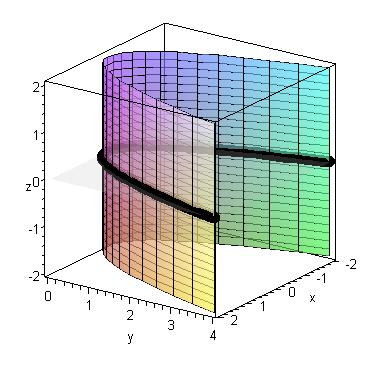
\includegraphics[width=\mywidth]{functions/cylinder-1}&
%%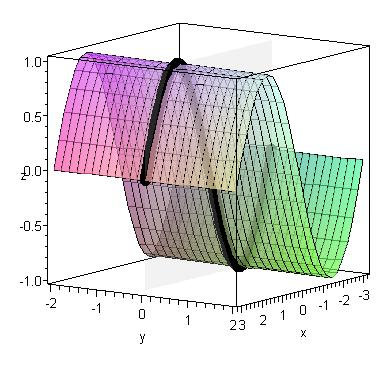
\includegraphics[width=\mywidth]{functions/cylinder-2}&
%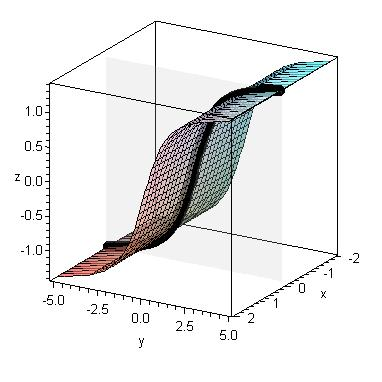
\includegraphics[width=\mywidth]{functions/cylinder-3}&
%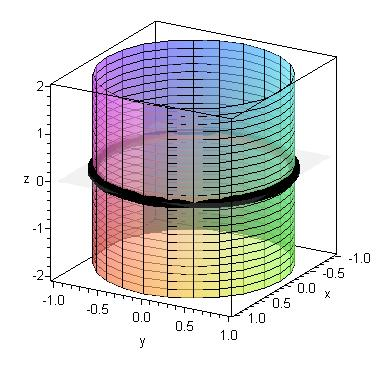
\includegraphics[width=\mywidth]{functions/cylinder-4}
\\
$y=\tan(z)$ &
$x^2+y^2=1$
\end{tabular}
\end{center}

\subsection{Quadric Surfaces}
A quadric surface is a generalization of a conic section to three
dimensions.  In general, it is the graph in 3D of any expression
involving at most second degree terms in $x$, $y$, and/or $z$. To
graph a quadric surface, hold one variable constant and then graph the
resulting conic section in the plane which represents the variable you
held constant. Repeat this for a few different variables and constants
until you can piece together the surface.  An example of this process
for $\frac{x^2}{4}+\frac{y^2}{9}-z^2 =1$ is illustrated below, as well
as some typical quadric surfaces.  \renewcommand{\mywidth}{.9in}
\begin{center}
\begin{tabular}{cccc}

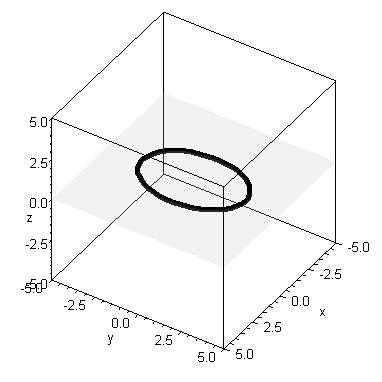
\includegraphics[width=\mywidth]{functions/quadric-1}&
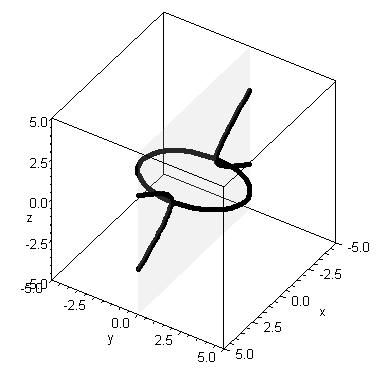
\includegraphics[width=\mywidth]{functions/quadric-2}&
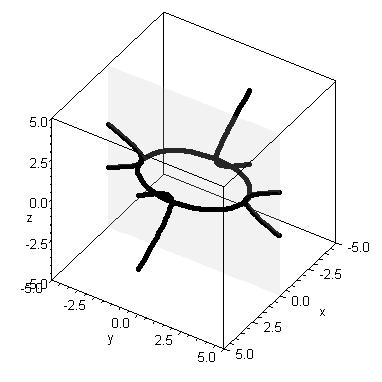
\includegraphics[width=\mywidth]{functions/quadric-3}&
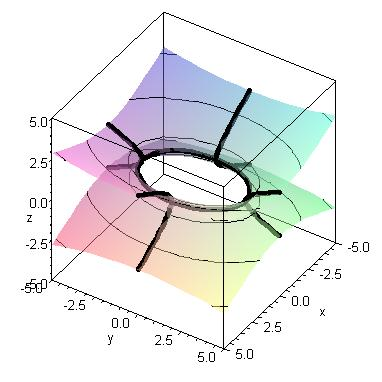
\includegraphics[width=\mywidth]{functions/quadric-4}
\\
Let $z=0$ &
Let $y=0$ &
Let $x=0$ &
$\frac{x^2}{4}+\frac{y^2}{9}-z^2 =1$\\
&&&Hyperboloid of one sheet
\\
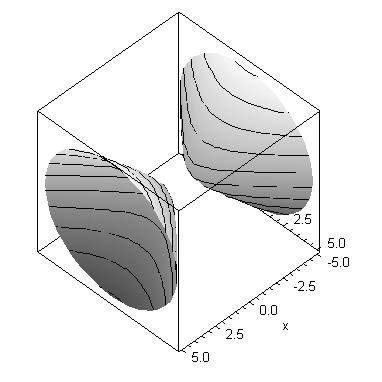
\includegraphics[width=\mywidth]{functions/quadric-5}&
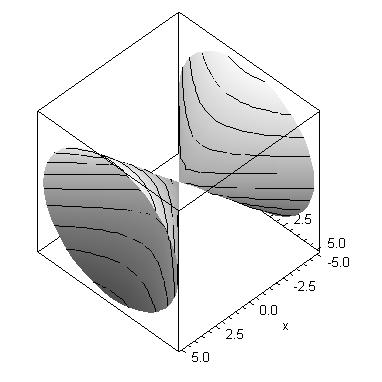
\includegraphics[width=\mywidth]{functions/quadric-6}&
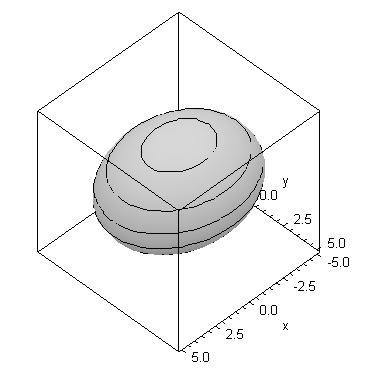
\includegraphics[width=\mywidth]{functions/quadric-7}&
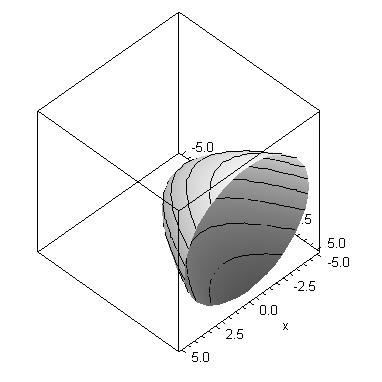
\includegraphics[width=\mywidth]{functions/quadric-8}
\\
$x^2-y^2-z^2=1$ &
$-x^2+y^2+z^2=0$ &
$\frac{x^2}{25}+\frac{y^2}{16}+\frac{z^2}{9}=1$ &
$x^2-4y+z^2=1$
\\
Hyperboloid of 2 sheets&
Cone &
Ellipsoid &
Paraboloid
\end{tabular}
\end{center}






\section{Function terminology}
A function is a set of instructions (a relation) involving two sets
(called the \emph{domain} and \emph{codomain}).  A function assigns to
each element of the domain $D$ at most one element in the codomain
$R$. It is customary to write {$f\colon D\to R$} when we want to
specify the domain and codomain.  Not all elements of $R$ may be
assigned; the set of elements in $R$ that are assigned is called the
\emph{range} or \emph{image} of the function.
\note{drawing of the domain, range, and codomain circles, with the function arrow going between}

\begin{example}
  If the function $f(x)=x^2$, then the domain and codomain are typically
  $\RR$ (i.e., $f\colon \RR \to \RR$), and the range is the set of nonnegative numbers.
\end{example}

In this class, we will study what happens when the domain and codomain
are subsets of {${\RR}^n$} ($\RR^n$ is the set of all $n$-dimensional
real points, and is often called ``Euclidean {$n$}-space''). In
particular we will study functions of the form $f\colon {\RR}^n\to
{\RR}^m$.

\section{Functions: $\RR^n\to \RR$}
\subsection{Functions of one variable: $f\colon \RR^1\to  \RR^1$}
In the first year of calculus, the domain and codomain are always
subsets of the real numbers {$\RR$}.  A typical example is $f(x)=x^2$.
Many ideas like derivatives, integrals, etc., from first semester
calculus generalize to all dimensions, but some do not.

\subsection{Functions of several variables: \\ $f\colon \RR^2\to \RR$, $f\colon \RR^3\to \RR$, $f\colon \RR^n\to \RR$} 

With functions of this type, the output dimension is always 1, while
the input dimension may be as large as needed. This type of function
is used to measure a quantity at each point in the plane ($f\colon {\RR}^2\to
{\RR}$), at each point in space ($f\colon {\RR}^3\to {\RR}$), or for every
combination of $n$ inputs ($f\colon {\RR}^n\to {\RR}$). The temperature at
each point in the plane would be modeled by such a function of the
form $T(x,y)$. The wind speed at each point in space could be modeled
by a function of the form $f(x,y,z)$.

To graph functions of the form {$f\colon {\RR}^2\to {\RR}$}, we typically
write $z=f(x,y)$ and then plot the function in $xyz$ coordinates.
Every pair $(x,y)$ corresponds to exactly one point $(x,y,f(x,y))$ in
space.  Functions of this form still pass the ``vertical line test''
(where ``vertical line'' means a line parallel to the $z$-axis).  We
get 2D traces (vertical cross sections) of the function by replacing
$x$ or $y$ with a constant and creating a 2D graph of the resulting
function.  A level curve is a graph in the plane of the equation
$c=f(x,y)$ for some constant $c$ (essentially a level curve is a
horizontal cross section drawn in the $xy$-plane). Plotting several
level curves creates a \emph{contour plot} of the function.  A few
graphs and corresponding contour plots follow.


\renewcommand{\mywidth}{1.1in}
\begin{center}
\begin{tabular}{ccccc}
\tikzsetfigurename{functions-}
\begin{tikzpicture} 
 \begin{axis}[footnotesize, view={60}{30}, colormap/blackwhite] 
   \addplot3[surf,domain=-3:3,y domain=-3:3] {9-x*x-y*y}; 
 \end{axis} 
 \end{tikzpicture}
&
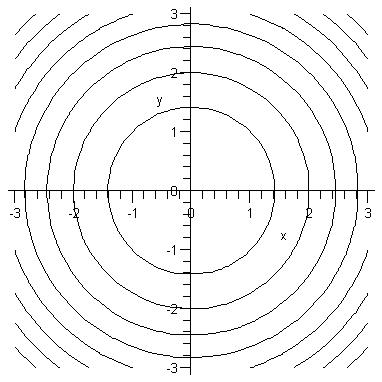
\includegraphics[width=\mywidth]{functions/functionseveral-2}&
\begin{tikzpicture} 
  \begin{axis}[footnotesize, view={60}{30}, colormap/blackwhite] 
    \addplot3[surf,domain=-2*pi:2*pi,y domain=-2*pi:2*pi] {sin(deg(x))*cos(deg(y))}; 
  \end{axis} 
\end{tikzpicture}&
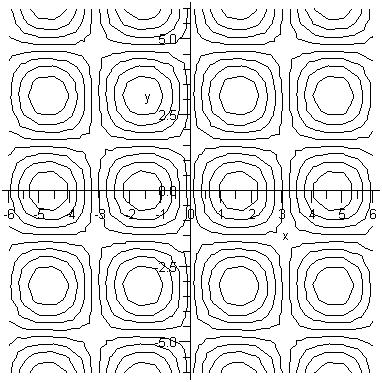
\includegraphics[width=\mywidth]{functions/functionseveral-4}
\\
$f(x,y)=9-x^2-y^2$&
level curves of $f$ &
$g(x,y) = \sin x \cos y$ &
level curves of $g$\end{tabular}
\end{center}

Functions with three inputs {$f\colon {\RR}^3\to {\RR}$} would require 4
dimensions to graph.  Rather than graph functions in 4D, we instead
look at level surfaces. For the function $w=f(x,y,z)$, we pick a
constant $w=c$ and graph the surface $c=f(x,y,z)$.  The level surface
$w=1$ for the function $f(x,y,z)=x^2+y^2+z^2$ is a sphere of radius 1
(given by graphing $x^2+y^2+z^2=1$).  Quadric surfaces will show up
often when you graph level surfaces of functions with three inputs.


\section{Parametric Functions}

\subsection{Parametric curves: {$\vec r\colon \RR\to \RR^2$}}
Parametric curves often represent motion in the plane.  We can write
these functions by giving the equations for each coordinate
separately, or we can write all of the equations as a vector, where
each coordinate of the vector is a function of one variable.  Because
the output of these functions is a vector, we call these functions
\emph{vector-valued functions}, and often emphasize this by writing
them with a vector symbol over the name.


\begin{example}
  The parametric curve $x=2\cos t$, $y=3\sin t$ traces out an ellipse.
  We can also write this in vector form as $\vec r(t) = \langle2\cos
  t, 3\sin t\rangle$.
\end{example}

\subsection{Spacecurves: {$\vec r\colon \RR\to \RR^3$}}
Space curves generalize parametric curves, but the outputs are
three-dimensional points, so these are curves in space.  The notation
{$\vec r\colon \RR \to \RR^3$} suggests that we are graphing a
one-dimensional object in three dimensions. The graph of a space curve
looks like a bent wire in space, or as a path of motion traced out in
space.  For each time $t$, the position vector $\vec r(t)$ gives the
position of a particle whose motion is described by the space curve.
Again, since the output is a vector, a space curve is a vector-valued
function.  Just like a 2D parametric plot, a space curve can graphed
by picking values for $t$ and plotting the corresponding points $\vec
r(t)$.

The derivative of a space curve is found by differentiating each
component of the space curve, which follows immediately by looking at
the limit $\ds\frac{d\vec r}{dt}=\lim_{h\to 0}\frac{\vec r(t+h)-\vec
  r(t)}{h}$. An equation of the tangent line to a space curve at $t=c$
has direction vector equal to $\dfrac{d\vec r}{dt}$ (evaluated at
$t=c$) and passes through the point $\vec r(c)$, and so has an equation of
$\vec l(u) = \vec r^\prime(c)u+\vec r(c)$. If a space curve is used to
describe motion, then velocity is $\vec v(t) = \dfrac{d\vec r}{dt}$,
speed is the magnitude of velocity $|\vec v|$, and acceleration is
$\vec a(t) = \dfrac{d\vec v}{dt}$, just as was taught in first-semester
calculus for single-variable functions.

\begin{example}
%\pgfplotsset{
%every axis style= {view/h=-45}}

\marginpartop{\begin{tikzpicture} 
    \begin{axis}[footnotesize, colormap/blackwhite, view/h=-40,
      xlabel=$x$, ylabel=$y$] 
      % tangent line
     \addplot3[mark=>] coordinates {(-0.0669872981077807, 1.11602540378444,
       1.59439510239320) (-0.933012701892219, 0.616025403784439,
       2.59439510239320)}; 
     % acceleration vector
     \addplot3[mark=>] coordinates {(-0.500000000000000, 0.866025403784439,
       2.09439510239320) (0.000000000000000, 0.000000000000000,
       2.09439510239320)};
     \addplot3[domain=0:4*pi, samples y=0, smooth] 
      ({cos(deg(x))}, {sin(deg(x))}, {x}); 
   \end{axis} 
  \end{tikzpicture}}%

% sage: r(t)=(cos(t), sin(t), t)
% sage: v=diff(r,t)(2*pi/3)
% sage: p=r(2*pi/3)
% sage: l=v*t+p
% sage: l(t=-0.5).n()
% (-0.0669872981077807, 1.11602540378444, 1.59439510239320)
% sage: l(t=0.5)
% (-0.250000000000000*sqrt(3) - 1/2, 1/2*sqrt(3) - 0.250000000000000, 2/3*pi + 0.500000000000000)
% sage: l(t=-0.5).n()
% (-0.0669872981077807, 1.11602540378444, 1.59439510239320)
% sage: a=diff(r,t,2)
% sage: print '%s %s'%(p.n(), (p+a(2*pi/3)).n())
% (-0.500000000000000, 0.866025403784439, 2.09439510239320) (0.000000000000000, 0.000000000000000, 2.09439510239320)


The space curve {$\vec r(t)=\langle\cos(t),\sin(t),t\rangle$} is a
helix which wraps around the $z$-axis.  Its graph is shown in the
margin, where $0\leq t\leq 4\pi$, as well as the tangent line and
acceleration vector. The velocity and acceleration at any time $t$ are
$\vec v(t) = \langle-\sin(t),\cos(t),1\rangle$ and $\vec a(t) =
\langle-\cos(t),-\sin(t),0\rangle$. When $t=2\pi/3$, we have $\vec
r(2\pi/3) = \langle1/2,\sqrt{3}/2,2\pi/3\rangle$, $\vec v(2\pi/3) =
\langle-\sqrt{3}/2,-1/2,1\rangle$, and $\vec a(2\pi/3) =
\langle1/2,-\sqrt{3}/2,0\rangle$. An equation of the tangent line is
$\vec l(t) = \vec v(2\pi/3)t+ \vec r(2\pi/3)=
\langle-\sqrt{3}/2,-1/2,1\rangle
t+\langle1/2,\sqrt{3}/2,2\pi/3\rangle$.
\end{example}


\subsection{Parametric Surfaces: {$\vec f\colon {\RR}^2\to {\RR}^3$} }

Just as parametric and space curves describe one-dimensional objects, we use parametric surfaces to describe two-dimensional objects in 3D.  Notice that we are mapping two dimensions into three, so think of a parametric surface as a set of instructions of how to place the 2D plane in space (where you can twist the plane and stretch it based on the set of instructions).  If you hold one variable constant, then the graph of the resulting function is a space curve. To graph a parametric surface, hold one variable constant and draw the resulting space curve.  Do this for a few values of each variable, and you will have created a net of overlapping space curves from which you can piece together the surface.  

Any surface of the form $z=f(x,y)$ can be made a parametric surface by
writing $\vec r(x,y)=\langle x,y,f(x,y)\rangle$, which just says for
each $(x,y)$ to plot the point $(x,y,f(x,y))$. We often use $u$ and
$v$ as variables for a parametric surface if those variables do not
represent some other standard quantity.

{
\tikzsetfigurename{parametricsurface-}
\begin{center}
\begin{tabular}{cccc}
\begin{tikzpicture} 
  \begin{axis}[footnotesize, view/h=-40,colormap/blackwhite] 
    \addplot3[surf,domain=-4:4,y domain=-4:4] 
    (x,y,{9-x^2-y^2}); 
  \end{axis} 
\end{tikzpicture}&

\begin{tikzpicture} 
  \begin{axis}[footnotesize, view/h=-40, colormap/blackwhite, z buffer=sort] 
    \addplot3[surf,domain=0:3,y domain=0:2*pi] 
    ({x*cos(deg(y))},{x*sin(deg(y))}, {9-x^2}); 
  \end{axis} 
\end{tikzpicture}\\
\parbox{0.5\textwidth}{\centering $\vec r(x,y) = \langle
  x,y,9-x^2-y^2\rangle$\\$-4\leq x\leq 4$, $-4\leq y\leq 4$}
&
\parbox{0.5\textwidth}{\centering $\vec r(u,v)=\langle u\cos v,u\sin v
  ,9-u^2\rangle$\\
  $0\leq u\leq 3$, $0\leq v\leq 2\pi$\\ 
  (cylindrical coordinates)}
\\[12pt]


\begin{tikzpicture} 
  \begin{axis}[footnotesize, view/h=-40, colormap/blackwhite, 
    z buffer=sort, variable=θ, variable y=φ] 
    \addplot3[surf,domain=0:2*pi,y domain=pi/4:3*pi/4] 
    ({3*cos(deg(θ))*sin(deg(φ))},{3*sin(deg(θ))*sin(deg(φ))},{3*cos(deg(φ))});
 \end{axis} 
\end{tikzpicture}&

\begin{tikzpicture} 
  \begin{axis}[footnotesize, view/h=-40, z buffer=sort, colormap/blackwhite] 
    \addplot3[surf,domain=0:2*pi,y domain=0:pi] 
    ({x*sin(deg(x))*cos(deg(y))},{x*cos(deg(x))*cos(deg(y))}, {x*sin(deg(y))}); 
  \end{axis} 
\end{tikzpicture}\\

\parbox{0.5\textwidth}{\centering $\vec
  r(\theta,\phi)=\langle3\cos\theta\sin\phi,3\sin\theta\sin\phi,3\cos\phi\rangle$\\
  $0\leq \theta\leq 2\pi$, $\frac{\pi}{4}\leq \phi\leq \frac{3\pi}{4}$
  \\
  (spherical coordinates) } 
&

\parbox{0.5\textwidth}{\centering $\vec r(u,v)=\langle u\sin u \cos v
  , u\cos u \cos v , u\sin v \rangle$\\
 $0\leq u\leq 2 \pi$, $0\leq v\leq \pi$}



\end{tabular}
\end{center}
}

\section{Functions: $\RR^n\to \RR^n$}

\subsection{Transformations (changing coordinates)\\ {$\vec f\colon \RR^2\to \RR^2$}, {$\vec f\colon \RR^3\to \RR^3$}}

The polar coordinate equations $x=r\cos\theta$, $y=r\sin\theta$
require two inputs $(r,\theta)$ and give two outputs $(x,y)$.  This can
be thought of as a function $T(r,\theta)=\langle
r\cos\theta,r\sin\theta\rangle$. Every time we change coordinate
systems, it will be valuable to give that tranformation a name and
recognize that it is really a function.

\note{drawing showing a transformation of the $r,\theta$ plane to the $x,y$ plane}

\subsubsection{Cylindrical Coordinates}
Cylindrical coordinates is an extension of polar coordinates to three
dimensions.  The transformation $T(r,\theta,z) = \langle
r\cos\theta,r\sin\theta,z\rangle$ gives us a new way of viewing points
in 3D.  Using the triangle $x,y,r$, we can figure out the following
relationships.
\begin{align*}
  x&=r \cos \theta & 
  y&=r \sin \theta & 
  \tan\theta&=y/x & 
  r^2&=x^2+y^2     
\end{align*}

\begin{example}
The cylindrical point {$(r, \theta, z)=(3,\pi/2,4)$} in
cylindrical coordinates is the same as the rectangular point $(x,y,z)
= (0,3,4)$.
\end{example}

\subsubsection{Spherical Coordinates}
Spherical coordinates $(\rho,\theta,\phi)$ are defined as follows.
The distance (\emph{radius}) from the origin to the point $(x,y,z)$ is
called $\rho$. The angle $\theta$ (the \emph{azimuth}) is the same as
in polar or cylindrical coordinates. The angle $\phi$ (the
\emph{inclination}) is the angle between the positive $z$-axis and a
ray from the origin to $(x,y,z)$. Using these definitions, we obtain
the following equations by considering the two right triangles with
edges $x,y,r$ and $r,z,\rho$:\note{draw nice pictures of the variables for cylindrical and spherical coordinates}
\begin{align*}
  x&=\rho\sin\phi\cos\theta  &
  y&=\rho\sin\phi\sin\theta & 
  z&=\rho\cos\phi\\
  \tan\theta&=y/x &
  r&=\rho\sin\phi & 
  \rho^2&=x^2+y^2+z^2 &
\end{align*}
We can describe the spherical coordinate transformation as a
function 
$$T(\rho,\theta,\phi) = \langle\rho\sin\phi\cos\theta,\rho\sin\phi\sin\theta,\rho\cos\phi\rangle.$$ 

\begin{example} 
The spherical point {$(\rho, \theta, \phi)=(4,\pi,\pi/4)$} is the same
as the rectangular point $(x,y,z) = (4/\sqrt{2},0,4/\sqrt{2})$.
\end{example}

There is some disagreement in different fields about the notation for
spherical coordinates.  In some fields, $\phi$ represents the azimuth
angle and $\theta$ represents the inclination angle (or the
\emph{elevation} angle---the angle from the $xy$-plane).
Additionally, sometimes the coordinates are written in a different
order.  You should always check the notation for spherical coordinates
before communicating using them.
\note{draw some nice plots illustrating the transformation in 3d}

\subsubsection{Graphing in other coordinate systems}
To graph an equation in a different coordinate system, simply substitute the equation into the transformation and graph the result as a parametric surface.  

\begin{example}
Suppose we have the spherical coordinate equation $\rho(\theta,\phi)=3\phi^2\cos\theta$.  Subsituting this in for $\rho$ in the transformation function gives 
\begin{align*}
T(\theta,\phi) &= \langle\rho(\theta,\phi)\sin\phi\cos\theta, \rho(\theta,\phi)\sin\phi\sin\theta, \rho(\theta,\phi)\cos\phi\rangle\\
&=\langle3\phi^2\cos\theta\sin\phi\cos\theta, 3\phi^2\cos\theta\sin\phi\sin\theta, 3\phi^2\cos\theta\cos\phi\rangle\\
\end{align*}
\end{example}
 
You can see two examples of graphing $z=9-r^2$ (cylindrical
coordinates, where $u=r$ and $v=\theta$) and $\rho=3$ (spherical
coordinates) in the parametric surfaces section.

\subsection{Vector Fields: {$\vec f\colon \RR^2\to \RR^2$}, {$\vec f\colon \RR^3\to \RR^3$}}
Another way to represent a function mapping $\RR^n\to\RR^n$ is as a
vector field.  A vector field $\vec F(x,y) = \langle
M(x,y),N(x,y)\rangle$ or $\vec F(x,y,z) = \langle
M(x,y,z),N(x,y,z),P(x,y,z) \rangle$ is a function which assigns to
each point in the plane (or space) a vector.  Vector fields are used
to model gravity, forces, velocity, wind, acceleration, electric
fields, and many other things in nature. For example, the speed and
direction of wind depends on location, so the velocity of wind can be
represented by drawing a bunch of vectors at different points on a
map.  Vector fields may be one of the most useful tools we have.  You
should practice creating vectors given a description. 

\begin{example} 
A vector field in the plane in which the vector at any
point is directed towards the origin and has magnitude equal to the
square of the distance to the origin is
$$\vec F(x,y) =
(x^2+y^2)\frac{\langle-x,-y\rangle}{\sqrt{x^2+y^2}}.$$ We constructed
the equation for the vector field by expressing the vector at the
point $(x,y)$ as a magnitude times a unit direction vector.  
\end{example}

To graph a vector field $\vec F(x,y) = \langle M,N\rangle$ in the
plane, at each point $(x,y)$, we draw the vector $\vec F(x,y)$ at the
point $(x,y)$. Since the vectors may be rather long, computers will
proportionally rescale all vectors so that the vectors fit in the
graph.

% \begin{sagesilent}
%   mathematica('myplot = VectorPlot[{y, -x}, {x, -3, 3}, {y, -3, 3}]')
%   mathematica('Export["%s/functions-mma/field-circle.pdf", myplot]' % os.getcwd())
% \end{sagesilent}
%\includegraphics[width=\mywidth]{functions-mma/field-circle}
\begin{sagesilent}
var('x,y,z')
r=sqrt(x^2+y^2+z^2)
\end{sagesilent}
\renewcommand{\mywidth}{1.4in}
\begin{center}
\begin{tabular}{cccc}
\sageplot[width=\mywidth]{plot_vector_field((-y,x), (x,-5,5),(y,-5,5),pivot='middle'),aspect_ratio=1,figsize=2} &
\sageplot[width=\mywidth]{plot_vector_field((2*x+y,x-y), (x,-5,5),(y,-5,5),pivot='middle'),aspect_ratio=1,figsize=2} &
\sageplot[width=\mywidth][png]{plot_vector_field3d((-x/r,-y/r,-z/r), (x,-5,5),(y,-5,5),(z,-5,5),colors='black')}&
\sageplot[width=\mywidth][png]{plot_vector_field3d((y,z,x), (x,-5,5),(y,-5,5),(z,-5,5),center_arrows=True,colors='black')}
\\
$\vec F(x,y)=\langle-y,x\rangle$&
$\vec F(x,y)=\langle2x+y,x-y\rangle$&
$\vec F(x,y,z)=\frac{\langle-x,-y,-z\rangle}{\sqrt{x^2+y^2+z^2}}$&
$\vec F=\langle y,z,x \rangle$
%$F=\langle-x+y,-yz+1,z\rangle$
\end{tabular}
\end{center}
\note{use the subfigure environment}








%%% Local Variables: 
%%% mode: latex
%%% TeX-master: "../multivariable-calculus"
%%% End: 






\newgeometry{left=1in,right=1in,top=1in,bottom=1in}
\newpage

\section{Preparation}

\subsection{Lesson Plans}

This chapter covers the following ideas. When you create your lesson plan, it should contain examples which illustrate these key ideas. Before you take the quiz on this unit, meet with another student out of class and teach each other from the examples on your lesson plan. 

% A list of objectives for the chapter
%\begin{enumerate}
%\item ...
%\end{enumerate}


\begin{enumerate}
\item Be able to describe cylinders and quadric surfaces in space.
\item Describe uses for function with varying input and output
  dimensions.  Be able to draw appropriate representations when the
  input and output dimensions are 3 or less. Recognize by name and
  graph the different types of functions, in particular parametric
  equations, space curves, functions of several variables, vector
  fields, transformations, and parametric surfaces.
\item Find derivatives of space curves, and use the derivative to find
  tangent lines to space curves.
\end{enumerate}


%%% Local Variables: 
%%% mode: latex
%%% TeX-master: "../multivariable-calculus"
%%% End: 
%$


%\subsection{Preparation Problems}

%Here are the preparation problems for this unit.

\subsection{Homework}

In the following list, the ``basic practice'' problems should be quick
problems to help you master the ideas.  The ``good problems'' will
require a little more work.  The theory and application problems are
ones that will challenge you more; make sure you do the problems from
this area to fully master the material.  

{\noindent \footnotesize \begin{tabular}{|p{1.35in}|c|p{1.2in}|p{1.2in}|p{1.5in}|l|}\hline
Topic &Sec &Basic Practice &Good Problems &Thy/App \\\hline
Surfaces & 11.6 & 1--16, 31--40 & 19--30, 41--44 & 53--54, 56, 63--66\\\hline
Vector-valued functions & 12.1 & 1--42 & 43--68 & 81--83, 89--92\\\hline
& 12.2 & 1--26 & &\\\hline
& 12.3 & 1--16 & & \\\hline
& 12.4 & 19--20 & & \\\hline
Several variables& 13.1 & 1--28, 31--42, 45--48, 57--60 & 29--30, 43--44, 49--56, 65--66, 69--74 & 61--64, 67--68, 75--92\\\hline
Transformations & 11.7 & 1--12, 29--40, 57--72 & 73--86 & 121--122, Derive equations for cylindrical and spherical coordinates\\\hline
Vector Fields & 15.1 & 1--20 & & \\\hline
Parametric surfaces & 15.5 & 1--4, 9--18 & & 46--48, 53--54\\\hline
\end{tabular}
}




%%% Local Variables: 
%%% mode: latex
%%% TeX-master: "../multivariable-calculus"
%%% End: 


%%% Local Variables: 
%%% mode: latex
%%% TeX-master: "../multivariable-calculus"
%%% End: 

\restoregeometry


%\backmatter

%\printindex








%\appendix
%
%\chapter{The First Appendix}
%
%The \verb"\appendix" command should be used only once. Subsequent appendices can
%be created using the Chapter command.
%
%\chapter{The Second Appendix}
%
%Some text for the second Appendix.
%
%This text is a sample for a short bibliography. You can cite a book by making use of
%the command \verb"\cite{KarelRektorys}": \cite{KarelRektorys}. Papers can be cited
%similarly: \cite{Bertoti97}. If you want multiple citations to appear in a single set
%of square brackets you must type all of the citation keys inside a single citation,
%separating each with a comma. Here is an example: \cite{Bertoti97, Szeidl2001,
%Carlson67}.
%
%\begin{thebibliography}{9}
%\bibitem {KarelRektorys}Rektorys, K., \textit{Variational methods in Mathematics,
%Science and Engineering}, D. Reidel Publishing Company,
%Dordrecht-Hollanf/Boston-U.S.A., 2th edition, 1975
%
%\bibitem {Bertoti97} \textsc{Bert\'{o}ti, E.}:\ \textit{On mixed variational formulation
%of linear elasticity using nonsymmetric stresses and displacements}, International
%Journal for Numerical Methods in Engineering., \textbf{42}, (1997), 561-578.
%
%\bibitem {Szeidl2001} \textsc{Szeidl, G.}:\ \textit{Boundary integral equations for
%plane problems in terms of stress functions of order one}, Journal of Computational and
%Applied Mechanics, \textbf{2}(2), (2001), 237-261.
%
%\bibitem {Carlson67}  \textsc{Carlson D. E.}:\ \textit{On G\"{u}nther's stress functions
%for couple stresses}, Quart. Appl. Math., \textbf{25}, (1967), 139-146.
%\end{thebibliography}
%


%\backmatter

%
%\chapter{Afterword}
%
%The back matter often includes one or more of an index, an afterword,
%acknowledgements, a bibliography, a colophon, or any other similar item. In
%the back matter, chapters do not produce a chapter number, but they are
%entered in the table of contents. If you are not using anything in the back
%matter, you can delete the back matter TeX field and everything that follows it.
\end{document}


%%% Local Variables: 
%%% mode: latex
%%% TeX-master: t
%%% End: 
